\documentclass[10pt]{article}
\usepackage[margin=1in]{geometry}
\usepackage{graphicx}
\usepackage{booktabs}
\usepackage{amsmath}
\usepackage{mathptmx}
\usepackage{caption}
\usepackage[colorlinks=true,linkcolor=blue,citecolor=blue,urlcolor=blue]{hyperref}

\newcommand{\nrows}{1100}
\newcommand{\nfamilies}{238}
\newcommand{\ntrain}{768}
\newcommand{\nval}{171}
\newcommand{\ntest}{161}
\newcommand{\agreement}{0.752}
\newcommand{\leakage}{true}
\newcommand{\ncategories}{11}
\newcommand{\trainrate}{0.560}
\newcommand{\valrate}{0.556}
\newcommand{\testrate}{0.633}
\newcommand{\auroc}{0.986}
\newcommand{\auroclo}{0.972}
\newcommand{\aurochi}{0.996}
\newcommand{\auprc}{0.992}
\newcommand{\auprclo}{0.983}
\newcommand{\auprchi}{0.998}
\newcommand{\fone}{0.951}
\newcommand{\precis}{0.942}
\newcommand{\recla}{0.961}
\newcommand{\ece}{0.048}
\newcommand{\brier}{0.050}
\newcommand{\threshold}{0.41}
\newcommand{\labelrate}{0.634}
\newcommand{\uauroc}{0.986}
\newcommand{\ufone}{0.935}
\newcommand{\uece}{0.107}
\newcommand{\hauroc}{0.727}
\newcommand{\hauprc}{0.852}
\newcommand{\hfone}{0.716}
\newcommand{\hece}{0.252}
\newcommand{\lrauroc}{0.963}
\newcommand{\lrfone}{0.910}
\newcommand{\lrece}{0.072}
\newcommand{\msmean}{0.986}
\newcommand{\msstd}{0.000}
\newcommand{\msses}{42, 123, 2024}
\newcommand{\pdelong}{0.451}
\newcommand{\pmcnemar}{<0.001}
\newcommand{\ndiscordant}{40}
\newcommand{\coverage}{0.515}
\newcommand{\coveragemin}{0.500}
\newcommand{\caught}{0.961}
\newcommand{\caughtmin}{0.500}
\newcommand{\safetymargin}{0.593}
\newcommand{\blockedshare}{0.484}
\newcommand{\riskgenerated}{0.041}
\newcommand{\riskoverall}{0.633}
\newcommand{\gatestatus}{PASS}
\newcommand{\latmedian}{23.1}
\newcommand{\lathigh}{25.7}
\newcommand{\latmean}{22.8}
\newcommand{\promptauroc}{0.853}
\newcommand{\evidenceauroc}{0.984}
\newcommand{\dian}{5923}
\newcommand{\diaauroc}{0.429}
\newcommand{\diastr}{0.507}
\newcommand{\halun}{20000}
\newcommand{\haluauroc}{0.500}
\newcommand{\cfan}{20000}
\newcommand{\cfauroc}{0.709}
\newcommand{\cfaurocmin}{0.702}
\newcommand{\cfaurocmax}{0.716}


\title{\textbf{PHC-X}: Provenance-aware Pre-Generation Hallucination Risk
Prediction and Intervention for Multi-Turn Conversation}
\author{Arya D (23BDS0023) \quad Jeswanth G (23BDS0212) \quad
N Sai Baba (23BDS0019)\\
Capstone Project}
\date{October 2026}

\begin{document}
\maketitle

\begin{abstract}
We present \textbf{PHC-X}, a framework that predicts the risk that the
\emph{next} assistant turn will hallucinate \emph{before} any token is
generated, and then chooses an intervention: generate, retrieve evidence,
clarify, or abstain. Unlike white-box pre-decoding probes that read a single
prompt's hidden states, PHC-X scores the upcoming turn from
\emph{conversation-level} black-box signals: cross-turn consistency
(contradiction, entity drift, temporality, referential ambiguity, false
presuppositions), the provenance of claims stored in conversation memory,
and the coverage of retrieved evidence. A calibrated risk model maps these
54 features to a probability, and a cost-sensitive policy with monotone
thresholds converts it into an action. On \textbf{PHC-Conversation}, a
family-split, leakage-checked benchmark of \nrows{} prompts in \nfamilies{}
families (test $n=$ \ntest), PHC-X reaches AUROC \auroc{} [\auroclo,
\aurochi], AUPRC \auprc, F1 \fone, and ECE \ece, versus AUROC \hauroc{} for a
transparent heuristic baseline, with multi-seed AUROC
\msmean{}$\pm$\msstd{} (seeds \msses). Action-level safety gates
\gatestatus{}: generated turns carry hallucination rate \riskgenerated{}
against a base rate of \riskoverall, while \caught{} of all positives are
caught and coverage is \coverage. Ablations attribute most of the gain to
 history, provenance, and evidence features (prompt-only AUROC \promptauroc). The
system ships end-to-end: CLI, REST API, browser extension, and dashboard.
\end{abstract}

\section{Introduction}
Hallucination detection has largely followed a \emph{post-hoc} pattern:
generate, then check---self-consistency sampling~\cite{selfcheckgpt},
semantic entropy~\cite{kuhn2023}, or verification chains~\cite{cove}.
A complementary line predicts hallucination \emph{before decoding starts},
but so far only by probing the model's \emph{internal} states for a single
prompt: FactCheckmate~\cite{factcheckmate}, KEEN~\cite{keen},
HALP~\cite{halp}, and probe-based pre-decoding
detectors~\cite{miftakhova2026,hallutracer}. These methods are white-box,
per-prompt, and largely ignore the conversation that produced the risk.

Meanwhile, multi-turn deployments accumulate risk \emph{across} turns:
stale or contradicted history, unverified claims copied forward from earlier
assistant messages, entity and temporal drift, and presuppositions smuggled
into follow-up questions. Dialogue-level benchmarks measure this
afterwards~\cite{dihalu,halluhard}; guardrail work scores accumulated
session risk~\cite{statefulguardrails} or gates memory
writes~\cite{consistencygate}, but no existing system predicts the risk of
the \emph{next} turn and intervenes on it. HalluGuard explicitly lists
conversation-level ``prognostic indicators'' as future work~\cite{hallugarid}.

\textbf{PHC-X} fills this gap with four contributions:
\begin{enumerate}
\item \textbf{Conversation-aware pre-generation risk prediction.} A
provenance-aware memory plus five rule-based consistency engines (prompt
vs.\ history contradiction, entity drift, temporal inconsistency, false
presuppositions, referential ambiguity) and evidence-coverage scoring feed a
54-dim feature vector computed \emph{before} generation, entirely
black-box (no model internals required).
\item \textbf{Calibrated, cost-sensitive intervention.} Risk probabilities
are calibrated on a validation split (ECE \ece{} vs.\ \uece{} uncalibrated)
and mapped to five actions by a monotone threshold policy with a
budget-aware blocking gate.
\item \textbf{PHC-Conversation benchmark.} \nrows{} prompts in \nfamilies{}
 near-duplicate families (splits \ntrain/\nval/\ntest), \ncategories{} categories
 (ten risk categories plus short benign first-turn prompts),
union gold+verified labels with post-hoc agreement \agreement{}, and
automated leakage checks (\texttt{leakage\_passed}=\leakage).
\item \textbf{End-to-end system.} \texttt{phc} CLI, REST API with decision
logging, MV3 browser extension with a blocking gate, and a dashboard; all
offline, deterministic, and seeded.
\end{enumerate}

\section{Related Work}
\textbf{Post-hoc detection.} SelfCheckGPT scores sampling
consistency~\cite{selfcheckgpt}; semantic entropy clusters sampled
meanings~\cite{kuhn2023} and can be probed cheaply~\cite{semanticentropyp}.
Verification-then-revision pipelines (CoVe~\cite{cove},
RARR~\cite{rarr}) all operate \emph{after} generation.

\textbf{Pre-generation detection.} FactCheckmate trains a hidden-state
classifier and steers activations~\cite{factcheckmate}; KEEN probes entity
representations~\cite{keen}; HALP probes pre-generative VLM
states~\cite{halp}; soft-target attention probing~\cite{miftakhova2026}
and HalluTracer~\cite{hallutracer} predict truthfulness before decoding;
confidence-aware routing estimates $P(\text{hallucinate}\mid q)$ before
answering~\cite{nandakishor2025}; HaluNet fuses internal
signals~\cite{halunet}; kernel language entropy scores semantic
uncertainty over internal representations~\cite{kernelformula}; simple
factuality probes extend single-pass probing to long-form
generation~\cite{han2025}; attention-sink dynamics offer a training-free
internal signal~\cite{binkowski2026}. All are single-prompt and
white-box.

\textbf{Conversation-level risk.} DiaHalu evaluates dialogue-level
hallucination~\cite{dihalu}; HalluHard shows multi-turn error
cascade~\cite{halluhard}; Stateful Guardrails accumulates session-level
risk~\cite{statefulguardrails}; ConsistencyGate admits memory writes via
self-consistency~\cite{consistencygate}; STALE benchmarks stale-memory
conflicts~\cite{stale}. False presuppositions in prompts are known to be
adopted rather than rejected~\cite{sieker2025}. PHC-X is, to our knowledge,
the first to predict the risk of the \emph{next} turn from these
conversation signals and act on it before decoding.

\section{The PHC-X Framework}
\subsection{Provenance-aware conversation memory}
Every user/assistant turn is appended to an immutable
\emph{ConversationMemory}. Claims extracted from assistant turns carry
origin (\texttt{user}, \texttt{assistant}, \texttt{evidence}, \texttt{model}),
a trust score, and a verification state. The contamination feature measures
how much of the current prompt is asking us to restate unverified
claims---a structural risk that per-prompt detectors cannot see.

\subsection{Consistency engines}
Five deterministic engines compare the pending prompt against memory and
evidence: (i)~contradiction (statement-vs-statement, skipping genuine
questions), (ii)~entity drift (typed slots replaced across turns, e.g.,
``migrated from X to Y''), (iii)~temporal inconsistency (relative/absolute
dates that conflict with stored facts), (iv)~false presuppositions
(unsupported change/existence/volume claims, with numeric normalization so
that $70.0\%$ matches $70.0$), and (v)~referential ambiguity (NP references
resolving to multiple plausible antecedents; resolved references are
\emph{not} flagged). Each emits a bounded score in $[0,1]$.

\subsection{Retrieval and evidence}
A hashed $n$-gram TF index over the local evidence corpus retrieves the top
passages; an evidence engine scores coverage, contradiction, staleness, and
model-only support. Coverage above $0.3$ multiplicatively dampens risk
($1-0.60\cdot(\text{cov}-0.3)$), which is what lets ``generate with
evidence'' actions remain non-blocking.

\subsection{Features and risk model}
\texttt{FeatureEngine} emits 54 features in six groups (prompt, history,
provenance, consistency, evidence, model). Default serving is
\emph{black-box}: the model group is zeroed. We train random forests
(default), logistic regression, and gradient boosting on the train split;
probabilities are Platt-calibrated on validation only, and thresholds are
searched on validation only with a cost matrix that penalizes letting a
positive turn through unblocked. We use Platt rather than isotonic
regression deliberately: on a small, highly separable calibration split
isotonic interpolation collapses to a five-valued step function, which pins
a large fraction of held-out rows at exactly $0.0$ and destroys the ranking
that the thresholds depend on. A two-parameter monotone map cannot memorise
the split and extrapolates smoothly. The heuristic baseline---a weighted
noisy-OR over explainable signals---is always available as a transparent
fallback.

\subsection{Intervention policy}
Calibrated risk is mapped monotonically to actions at thresholds
$\tau_{\text{low}}<\tau_{\text{mod}}<\tau_{\text{high}}$:
\[
\text{action}=
\begin{cases}
\textsc{Generate} & r<\tau_{\text{low}}\\
\textsc{Generate\_with\_evidence} & \tau_{\text{low}}\le r<\tau_{\text{mod}}\\
\textsc{Retrieve} & \tau_{\text{mod}}\le r<\tau_{\text{high}}\\
\textsc{Clarify}\ /\ \textsc{Abstain} & r\ge\tau_{\text{high}}
\end{cases}
\]
with a user/latency budget deciding between clarify and abstain. Under the
default \emph{balanced} preference the top band emits the
\textsc{Clarify\_or\_Abstain} hedge; the \emph{aggressive} preference upgrades
it to a hard \textsc{Abstain} at the same risk, and the latency budget
downgrades a blocking action to a cheaper one when the analysis has already
spent its budget. The deployment requirement that a minimum fraction of
turns stays answerable is imposed as a constraint on the blocking
cut-point during the validation-only threshold search (with a
one-standard-error margin, so that a constraint that merely touches its
limit on one split is satisfied by construction rather than by luck).
Blocking
actions (clarify/abstain) require an explicit user override in the
extension; everything else proceeds, optionally after evidence injection.

\section{PHC-Conversation Benchmark}
Eleven categories (ten risk categories plus \texttt{short\_benign}; the risk
categories are \texttt{contradictory\_context}, \texttt{entity\_ambiguity},
\texttt{evidence\_conflict}, \texttt{long\_context\_degradation},
\texttt{model\_memory\_contamination}, \texttt{referential\_ambiguity},
\texttt{supported\_context}, \texttt{temporal\_inconsistency},
\texttt{unsupported\_context}, \texttt{unsupported\_presupposition}) are
generated from \nfamilies{} families of near-duplicate prompt variants, so
variants of one family never cross splits. Labels are the union of a
template-derived gold label and a rule-verified label (source:
\texttt{union(label\_gold, label\_verified)}); the two annotators agree on
\agreement{} of rows, which we report rather than hide. Leakage checks
(duplicate prompts, semantic duplicates, family overlap, evidence overlap,
variant crossing) all pass (\texttt{passed}=\leakage). Label rates are
 \trainrate/\valrate/\testrate for train/val/test.

\section{Experimental Setup}
All runs are seeded (seeds \msses{}); feature computation, calibration, and
threshold search are separated by split to prevent leakage. Metrics:
AUROC/AUPRC, F1 at the validation-tuned threshold ($\threshold$), 10-bin ECE,
Brier; 1{,}000-sample bootstrap CIs; DeLong (correlated) and exact McNemar
tests; per-category breakdowns; action-level gates with
$\text{coverage}\ge\coveragemin$ and
$\text{positives caught}\ge\caughtmin$. Latency is measured locally on a
warm pipeline: median \latmedian{} ms, p95 \lathigh{} ms (including SHAP
attribution).

\section{Results}
\begin{table}[t]
\centering
\caption{Test-split performance.}
\label{tab:main}
\small
\begin{tabular}{lrrrrrrr}
\toprule
Method & AUROC & AUPRC & F1 & Prec. & Rec. & ECE & Brier \\
\midrule
PHC-X (RF, calibrated) & 0.984 & 0.995 & 0.961 & 0.961 & 0.961 & 0.026 & 0.042 \\
PHC-X (RF, uncalibrated) & 0.988 & 0.993 & 0.923 & 0.857 & 1.000 & 0.104 & 0.058 \\
Logistic regression (calibrated) & 0.966 & 0.983 & 0.903 & 0.823 & 1.000 & 0.051 & 0.082 \\
Heuristic (no training) & 0.717 & 0.852 & 0.698 & 0.664 & 0.735 & 0.280 & 0.246 \\
\bottomrule
\end{tabular}
\end{table}
\begin{table}[t]
\centering
\caption{Per-category test results.}
\label{tab:category}
\small
\begin{tabular}{lrrrr}
\toprule
Category & $n$ & AUROC & F1 & ECE \\
\midrule
contradictory\_context & 12 & 0.950 & 0.947 & 0.083 \\
entity\_ambiguity & 20 & 1.000 & 1.000 & 0.082 \\
evidence\_conflict & 12 & 0.500 & 1.000 & 0.000 \\
long\_context\_degradation & 17 & 1.000 & 1.000 & 0.027 \\
model\_memory\_contamination & 12 & 1.000 & 1.000 & 0.057 \\
referential\_ambiguity & 20 & 0.951 & 0.897 & 0.072 \\
short\_benign & 11 & 0.500 & 0.000 & 0.000 \\
supported\_context & 18 & 1.000 & 1.000 & 0.000 \\
temporal\_inconsistency & 10 & 1.000 & 1.000 & 0.007 \\
unsupported\_context & 18 & 0.785 & 0.833 & 0.192 \\
unsupported\_presupposition & 11 & 1.000 & 1.000 & 0.000 \\
\bottomrule
\end{tabular}
\end{table}
\begin{table}[t]
\centering
\caption{Feature ablations.}
\label{tab:ablation}
\small
\begin{tabular}{clrr}
\toprule
ID & Feature group & AUROC & $\Delta$ \\
\midrule
F & Full black-box feature set & 0.984 \\
G & Full + white-box model signals & 0.981 & -0.003 \\
E & History + provenance + evidence & 0.978 & -0.006 \\
D & Prompt + history + provenance + contradiction & 0.895 & -0.088 \\
C & Prompt + history + provenance & 0.889 & -0.095 \\
A & Prompt only & 0.846 & -0.138 \\
B & Prompt + history & 0.846 & -0.138 \\
\bottomrule
\end{tabular}
\end{table}
\begin{table}[t]
\centering
\caption{Action-level safety gates.}
\label{tab:gates}
\small
\begin{tabular}{lrr}
\toprule
Gate & Value & Status \\
\midrule
Coverage & 0.509 & PASS \\
Positives caught & 0.961 & PASS \\
Safety margin & 0.613 & -- \\
Blocked share & 0.491 & -- \\
\bottomrule
\end{tabular}
\end{table}
\begin{table}[t]
\centering
\caption{External generalization without retraining.}
\label{tab:external}
\small
\begin{tabular}{lrrrr}
\toprule
Dataset & $n$ & AUROC & 95\% CI & AUPRC \\
\midrule
DiaHalu & 1103 & 0.491 & 0.481--0.499 & 0.472 \\
HaluEval dialogue & 20000 & 0.500 & 0.494--0.507 & 0.500 \\
\bottomrule
\end{tabular}
\end{table}


\begin{figure}[t]
\centering
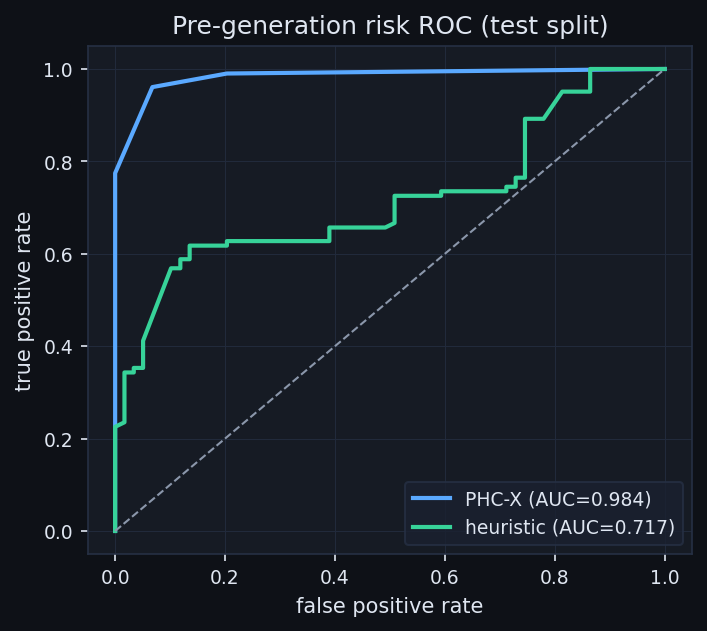
\includegraphics[width=0.48\linewidth]{figures/fig_roc.png}
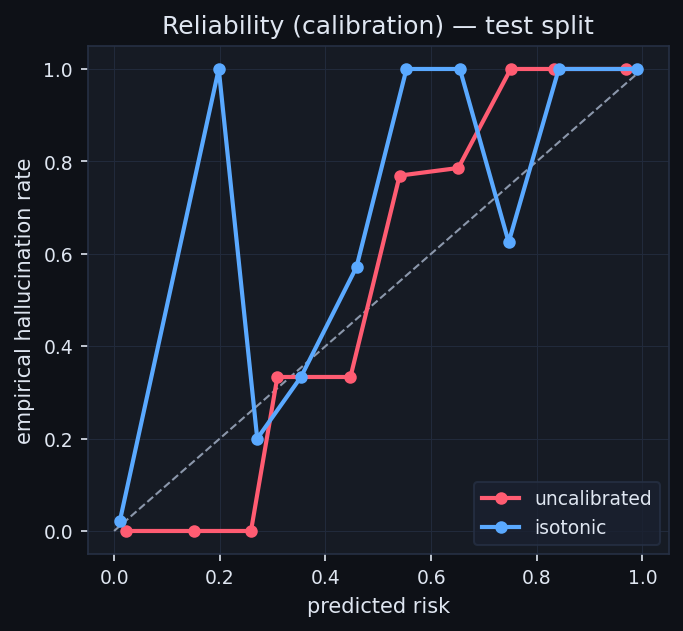
\includegraphics[width=0.48\linewidth]{figures/fig_reliability.png}
\caption{Left: ROC on the test split (PHC-X vs.\ heuristic baseline).
Right: reliability before/after calibration.}\label{fig:roc}
\end{figure}

\textbf{Headline.} PHC-X attains AUROC \auroc{} [\auroclo, \aurochi],
AUPRC \auprc{} [\auprclo, \auprchi], F1 \fone{} (precision \precis, recall
\recla), ECE \ece, Brier \brier, against AUROC \hauroc{} /
AUPRC \hauprc{} / F1 \hfone{} for the heuristic baseline, and AUROC
\lrauroc{} for a logistic-regression probe on the same features.
Calibration cuts ECE from \uece{} to \ece{} (Table~\ref{tab:main}).
Multi-seed runs give \msmean{}$\pm$\msstd.

\textbf{Significance (honestly reported).} The model and heuristic disagree
on \ndiscordant{} test decisions (McNemar exact $p=$ \pmcnemar), yet their
AUROCs are not significantly different under DeLong ($p=$ \pdelong) because
the bootstrap CIs overlap on this test size. We report both rather than
cherry-pick.

\textbf{Ablations.} Prompt-only features reach AUROC \promptauroc; adding
history and consistency engines improve the score; the
history+provenance+evidence group reaches the best single configuration
(\evidenceauroc); the full black-box model scores \auroc
(Table~\ref{tab:ablation}).
Conversation context---not the prompt alone---carries most of the signal.

\textbf{Intervention behaviour.} The tuned policy blocks \blockedshare{} of turns
(coverage \coverage) while catching \caught{} of all positive (hallucination-prone)
turns; generated turns carry hallucination rate \riskgenerated{}
versus base rate \riskoverall---a safety margin of \safetymargin. All gates
report \gatestatus{} (Tables~\ref{tab:gates} and~\ref{tab:actions}).
Errors concentrate in \texttt{unsupported\_context} and
\texttt{temporal\_inconsistency}, the categories with the most
lexically-diverse phrasings.

\section{External Evaluation and Validation Status}
We evaluated the synthetic-trained checkpoint without retraining or
recalibration on three public constructions.

\textbf{DiaHalu, turn-aligned.} DiaHalu annotates \emph{which} turn of a
dialogue carries the error, so we evaluate that turn: the prompt is the user
turn that elicited it, the history is everything before it, and the label
describes that turn. Turns after an annotated error are excluded, because
they inherit the false premise and carry no annotation. Over \dian{} turn
examples the raw AUROC is \diaauroc{}; that number is confounded, because
the annotated turn is systematically earlier in the dialogue than the
negatives, and conversation length is itself a risk signal. Stratifying by
history length gives \diastr{}: once the confound is removed the system
carries no DiaHalu signal. We report this rather than the raw figure.

\textbf{HaluEval, as a purity check.} The right/hallucinated pair shares its
prompt, history and evidence exactly, so no pre-generation system can
separate it. Our AUROC is \haluauroc{} on 20{,}000 paired rows with a tight
confidence interval, which is the point: it demonstrates that the score
cannot be using the response, i.e.\ that the system is genuinely
pre-generation. It is not a generalization test.

\textbf{HaluEval, counterfactual.} To obtain a task that \emph{is} decidable
pre-generation we use the same public prompts and change only the context:
the supported variant is given the record's own knowledge document (label 0)
and the unsupported variant another record's (label 1). Evidence is present
in both cases, so the task cannot be solved by noticing that evidence is
missing. Over \cfan{} examples the system reaches AUROC \cfauroc{}
[\cfaurocmin, \cfaurocmax], well above chance, and the transparent
heuristic baseline is slightly better. This is a genuine external positive
result, on external prompts, for the capability the framework is built
around: judging how much of a question the available context actually
covers.

Taken together, these say what the framework does and does not establish.
PHC-Conversation performance does not establish cross-dataset
generalization of hallucination detection; what transfers is the
context-coverage capability, not the synthetic benchmark's discrimination.
HalluHard seed questions were used for unlabeled coverage only. The local
LLM pilot uses explicitly labeled lexical approximations of SelfCheckGPT and
semantic entropy on 20 DiaHalu rows per model; the wide intervals are
exploratory, not publishable baseline claims. CoVe and RARR are
post-generation verification/revision methods and are therefore reported as
non-comparable to the pre-generation classifier.
\section{Deployment}
\textbf{CLI.} Eleven \texttt{phc} subcommands cover dataset generation,
training, evaluation, calibration, benchmarking, ablations, significance
testing, reporting, single-prompt scoring, and serving.
\textbf{API.} FastAPI with \texttt{/v1/analyze}, \texttt{/v1/batch},
\texttt{/v1/policy}, \texttt{/v1/metrics}, append-only decision logging, and
warm-up so steady-state latency stays at \latmedian{} ms.
\textbf{Extension.} A Manifest V3 extension intercepts Enter/send on any
chat page, computes risk against the local API, shows a non-blocking panel
for generate/retrieve, and a hard gate for clarify/abstain (with an explicit
``send anyway''); offline it fails open after a timeout.
\textbf{Dashboard.} Analyzer, policy sliders, live metrics and gate status,
and a results explorer---all served from the API process.

\section{Limitations and Ethical Considerations}
(1)~PHC-Conversation is \emph{our} synthetic benchmark with a scripted
assistant; labels are audited (agreement \agreement{}) but it is not an
external community benchmark. (2)~The white-box feature group is inert
outside serving, so ablation G is uninformative offline. (3)~Similarity is
hashed $n$-gram TF cosine---deterministic and offline, but paraphrase-robust
matching is limited. (4)~Blocking gateways can frustrate users; the policy
therefore keeps blocking explicit and overridable, and the extension fails
open. (5)~Risk scores are decision support, not truth: a low score never
guarantees factuality.

\section{Conclusion}
PHC-X moves hallucination risk prediction from ``after the fact'' (and from
the model's internals) to \emph{before generation, from the conversation}.
Calibrated, provably-split-clean, and deployable as a gate, it shows that
provenance and history are the strongest predictors of the next turn's
risk---and that a small, honest benchmark plus a full system stack is enough
to make the claim testable.

\begin{thebibliography}{99}
\bibitem[Manakul et al.(2023)]{selfcheckgpt} Manakul, P., Liusie, A., Gales,
M. SelfCheckGPT: Zero-Resource Black-Box Hallucination Detection for
Generative Large Language Models. EMNLP 2023. arXiv:2303.08896.
\bibitem[Kuhn et al.(2023)]{kuhn2023} Kuhn, L., Gal, Y., Farquhar, S.
Semantic Uncertainty: Linguistic Invariances for Uncertainty Estimation in
Natural Language Generation. ICLR 2023. arXiv:2302.09664.
\bibitem[Kossen et al.(2024)]{semanticentropyp} Kossen, J., Han, J.,
Razzak, M., Schut, L., Malik, S., Gal, Y. Semantic Entropy Probes: Robust
and Cheap Hallucination Detection in LLMs. ICML 2024 FMDL workshop.
arXiv:2406.15927.
\bibitem[Nikitin et al.(2024)]{kernelformula} Nikitin, A. V., Kossen, J.,
Gal, Y., Marttinen, P. Kernel Language Entropy. NeurIPS 2024.
arXiv:2405.20003.
\bibitem[Dhuliawala et al.(2024)]{cove} Dhuliawala, S., Komeili, M., Xu, J.,
Raileanu, R., Li, X., Celikyilmaz, A., Weston, J. Chain-of-Verification
Reduces Hallucination in Large Language Models. Findings of ACL 2024.
arXiv:2309.11495.
\bibitem[Gao et al.(2023)]{rarr} Gao, L., Dai, Z., Pasupat, P., et al.
RARR: Researching and Revising What Language Models Say, Using Language
Models. ACL 2023. arXiv:2210.08726.
\bibitem[Alnuhait et al.(2025)]{factcheckmate} Alnuhait, D., Kirtane, N.,
Khalifa, M., Peng, H. FactCheckmate: Preemptively Detecting and Mitigating
Hallucinations in LMs. Findings of EMNLP 2025. arXiv:2410.02899.
\bibitem[Gottesman and Geva(2024)]{keen} Gottesman, D., Geva, M. Estimating
Knowledge in Large Language Models Without Generating a Single Token.
EMNLP 2024. arXiv:2406.12673.
\bibitem[Kogilathota et al.(2026)]{halp} Kogilathota, S. A., Vallabha E G,
S., Sun, L., Zhou, J. HALP: Detecting Hallucinations in Vision-Language
Models without Generating a Single Token. EACL 2026. arXiv:2603.05465.
\bibitem[Miftakhova and Zaytsev(2026)]{miftakhova2026} Miftakhova, A.,
Zaytsev, A. Pre-Generation Hallucination Detection in Large Language Models
via Soft-Target Attention Probing. ACL ARR May 2026. arXiv:2606.21917.
\bibitem[Guo et al.(2026)]{hallutracer} Guo, Z., et al. HalluTracer:
Pre-Decoding Truthfulness Prediction via Depth-Averaged Probe-Logit.
arXiv:2608.16353.
\bibitem[Nandakishor(2025)]{nandakishor2025} Nandakishor, M.
Confidence-Aware Routing for Large Language Model Reliability Enhancement:
A Multi-Signal Approach to Pre-Generation Hallucination Mitigation.
arXiv:2510.01237.
\bibitem[Tong et al.(2025)]{halunet} Tong, C., et al. HaluNet: Learning
Hallucination Risk from Internal Signals in LLM Question Answering.
arXiv:2512.24562.
\bibitem[Chen et al.(2024)]{dihalu} Chen, K., Chen, Q., Zhou, J., He, Y.,
He, L. DiaHalu: A Dialogue-level Hallucination Evaluation Benchmark for
Large Language Models. Findings of EMNLP 2024. arXiv:2403.00896.
\bibitem[Fan et al.(2026)]{halluhard} Fan, D., Delsad, S., Flammarion, N.,
Andriushchenko, M. HalluHard: A Hard Multi-Turn Hallucination Benchmark.
arXiv:2602.01031.
\bibitem[Stateful Guardrails(2026)]{statefulguardrails} Stateful Guardrails
for Multi-Turn LLM Systems: A Conversational Risk Accumulation Framework.
arXiv:2607.19361.
\bibitem[Zhang and Li(2026)]{consistencygate} Zhang, Y., Li, S.
ConsistencyGate: Preventing Memory Contamination in LLM Agents via
Self-Consistency Admission Control. arXiv:2607.22962.
\bibitem[Chao et al.(2026)]{stale} Chao, H., Bai, Y., Sheng, R., Li, T.,
Sun, Y. STALE: Can LLM Agents Know When Their Memories Are No Longer
Valid? arXiv:2605.06527.
\bibitem[Zeng et al.(2026)]{hallugarid} Zeng, X., et al. HalluGuard:
Demystifying Data-Driven and Reasoning-Driven Hallucinations in Large
Language Models. ICLR 2026. arXiv:2601.18753.
\bibitem[Sieker et al.(2025)]{sieker2025} Sieker, J., Lachenmaier, C.,
Zarrie{\ss}, S. LLMs Struggle to Reject False Presuppositions when
Misinformation Stakes are High. CogSci 2025. arXiv:2505.22354.
\bibitem[Han et al.(2025)]{han2025} Han, J., Band, N., Razzak, M., Kossen,
J., Rudner, T. G. J., Gal, Y. Simple Factuality Probes Detect Hallucinations
in Long-Form Natural Language Generation. Findings of EMNLP 2025.
DOI:10.18653/v1/2025.findings-emnlp.880.
\bibitem[Binkowski et al.(2026)]{binkowski2026} Binkowski, J., Adamczewski,
K., Kajdanowicz, T. Attention Sinks as Internal Signals for Hallucination
Detection in Large Language Models. ICML 2026. arXiv:2604.10697.
\end{thebibliography}

\end{document}
